\chapter{System Maintenance}

\section{Environment}

\subsection{Software}
During the implementation of Markbook, I used following tools and software to help myself to create the system:
\begin{itemize}
    \item GitEye - alternative to GitHub, allows to push and pull files after updating my code to an online storage located on www.github.com, which is where I have my repository stored
    \item Python 3.4.1 - the actual programming language
    \item IDLE - user interface to write python code in 
    \item PyQt module - to use its features for python to create a graphical user interface
    \item SQLite Inspector - to view data stored in the database, also to test SQL queries before I implemented them to Markbook
    \item Google Chrome - as a web browser for additional documentation for Python and PyQt (such as http://pyqt.sourceforge.net/Docs/PyQt4/)
\end{itemize}

\subsection{Usage Explanation}
\begin{center}
    \begin{tabular}{|p{5cm}|p{5cm}|}
        \hline
        \textbf{Software} &  \textbf{Explanation}\\ \hline
GitEye & I did not have any other choice but to use GitEye to push, commit and pull my repositories to a cloud storage service located on github.com, when using college computers, so I had to stick to it.
\\ \hline
Python 3.4.1 & The reason why I chose python is because it's very simple to learn and I learned basics of it in the first year of A level computing.
\\ \hline
IDLE & I chose IDLE because it automatically is installed when python is installed. Also, IDLE is a text editor for python I was taught to use in the first year of computing.
\\ \hline
PyQt 4 & I chose PyQt 4 because of its high reputation; it is one of the most popular Python bindings. Additionally, I learned basics of PyQt at the end of first year of computing, so I knew that its features are more than satisfactory for this task.
\\ \hline
SQLite Inspector & My computing teacher, Adam, created this tool primarily for students working on this project, it has all and only features I need when handling database files. This makes it very easy to learn, as the amount of features is minimum.
\\ \hline
Google Chrome & I needed a web browser to search and access documentation for python and PyQt during the implementation. Google Chrome out of my experience is the fastest and crashes the least out of all browsers I had an opportunity to use.
\\ \hline
    \end{tabular}
\end{center}
\subsection{Features Used}
\begin{center}
    \begin{tabular}{|p{2cm}|p{8cm}|}
        \hline
        \textbf{Software} &  \textbf{Features Used}\\ \hline
        \hline
GitEye & I used GitEye's push, commit, pull and revert to previous commit.
        \\ \hline
Python 3.4.1 & 
        \\ \hline
IDLE & I used IDLE to write my python code using it and also run it. Additionally, to strucure the code, I used automatic indent, dedent, colour coded text and annotations to explain code. 
        \\ \hline
PyQt 4 & I used PyQt 4 to create the graphical user interface for Markbook. In specific, I used QtCore, QtGui and QtSql.  
        \\ \hline
SQLite Inspector & I used SQLite Inspector to view data and entity descriptions stored in sql databases. Also, I used it to view test queries before implementing them to the Markbook.
       \\ \hline
Google Chrome & Used to display web pages, so that I could view documentation for Python and PyQt.
\\ \hline
    \end{tabular}
\end{center}


\section{System Overview}
\textbf{Command Line Interface}
The Command Line Interface I created was primarily for testing purposes. It allows to  add, delete and amend data in the database file. Its interface is based on text.

\textbf{Graphical User Interface}
To make Markbook use more pleasant, a graphical interface is used to navigate between different sections of Markbook and access its features. For navigation, a menu bar with buttons is included at the top of the window. To provide additional information and help the user, a status bar is going to be included in future releases bottom of the window. To insert data, spinboxes and line edits are included. To trigger actions, buttons are included.

%use as many subsections as necessary for the system components
\subsection{System Component}
\section{Code Structure}
\subsection{File Explanation}

\begin{itemize}
    \item assignments_widget.py - for AssignmentsWidget class
    \item classes_widget.py for ClassStudents class
    \item classStudents_widget.py - for ClassStudents class
    \item classUnits_widget.py - for ClassUnits class
    \item studentAssignmentResults_widget.py - for StudentAssignments class
    \item students_widget.py for Students class
    \item teachers_widget.py for Teachers class
    \item unitAssignments_widget.py for Assignments class
    \item units_widget.py - for Units class
    \item basic_widgets.py - for StartWidget, InputDBNameWidget, ManagementWidget classes
    \item main_window.py - for the skeleton section of Markbook (all settings and layouts are initialized under MainWindow(QMainWindow)
    \item SQLConnection - for SQLConnection class (it is responsible for connection with a database file, so that data could be entered and extracted from the database)
    \item table_widget.py - for DisplayTableWidget class - generic class for a table, so that data could be presented with the use of it. It is unused, although it will be in future releases of Markbook
\end{itemize}


%use as many subsections as necessary for the code sections
\subsection{Particular Code Section}
%the code below can be uncommented and used to get a code section from a particular file
\begin{comment}

\end{comment}

\section{Variable Listing}
\section{System Evidence}

\subsection{User Interface}
\begin{figure}[H]   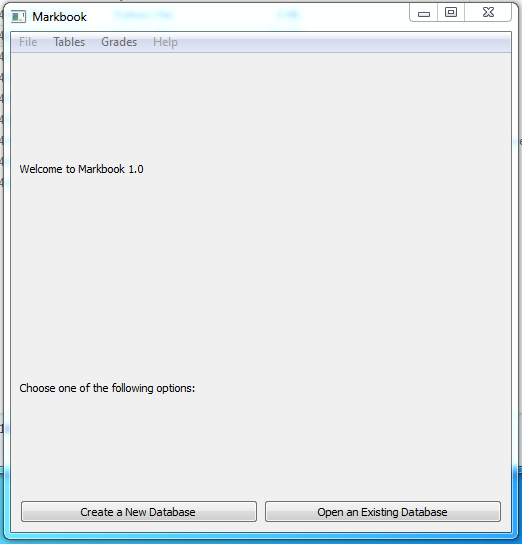
\includegraphics[width=\textwidth]{./Images/Initial Interface.png}
    \caption{Initial Interface} \label{}
\end{figure}

\begin{figure}[H]   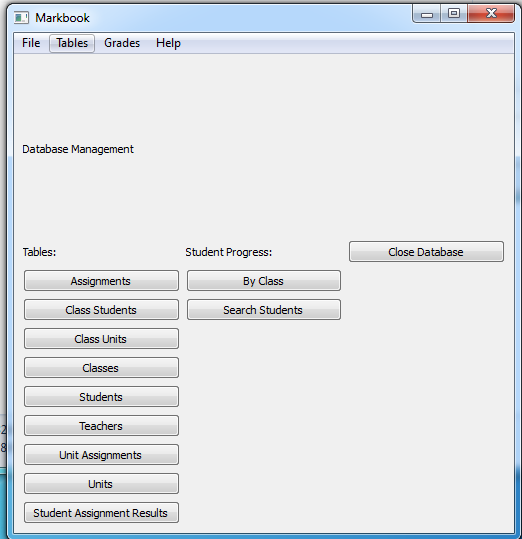
\includegraphics[width=\textwidth]{./Images/db_open.png}
    \caption{When database is opened interface} \label{}
\end{figure}

\begin{figure}[H]
    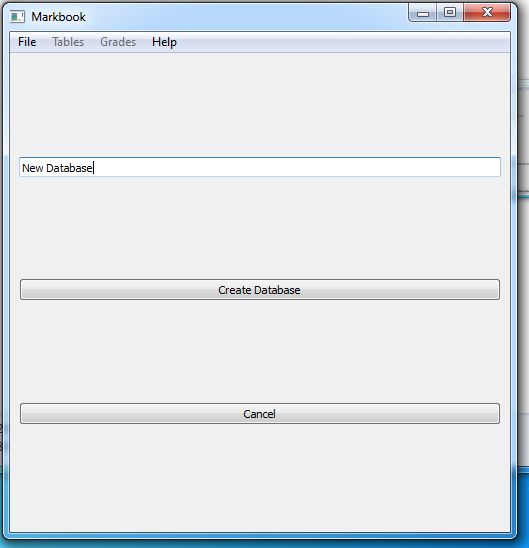
\includegraphics[width=\textwidth]{./Images/new_db.png}
    \caption{Interface for creating new database (although this does not function correctly)} \label{}
\end{figure}

\begin{figure}[H]
    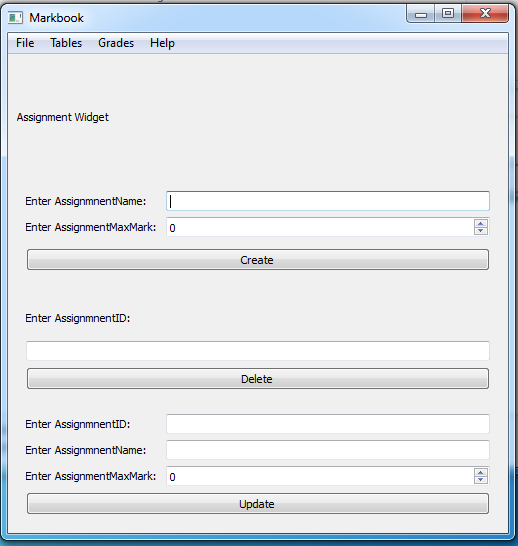
\includegraphics[width=\textwidth]{./Images/assignments.png}
    \caption{Assignments Widget} \label{}
\end{figure}

\begin{figure}[H]
    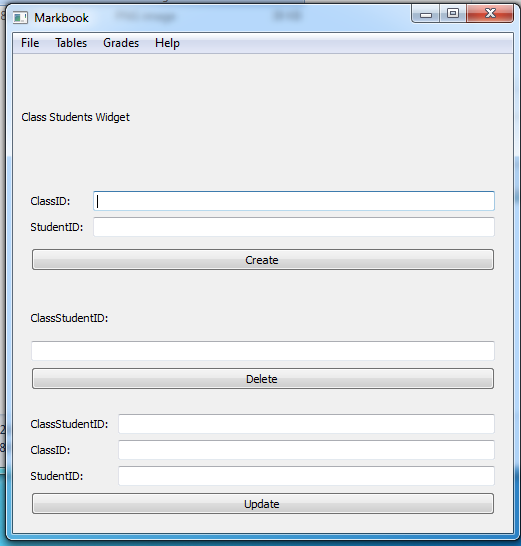
\includegraphics[width=\textwidth]{./Images/class students.png}
    \caption{Class Students Widget} \label{}
\end{figure}

\begin{figure}[H]
    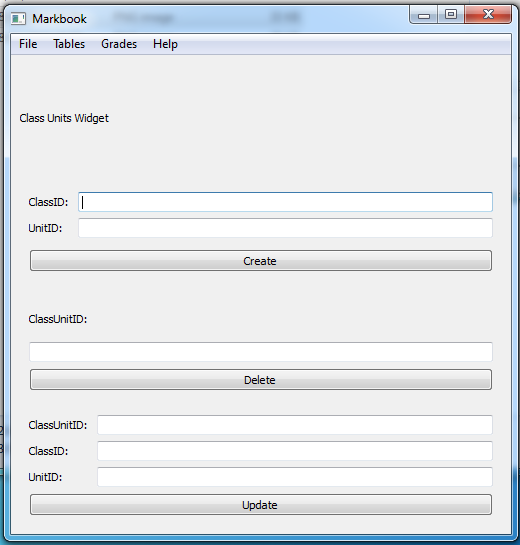
\includegraphics[width=\textwidth]{./Images/class units.png}
    \caption{Class Units Widget} \label{}
\end{figure}

\begin{figure}[H]
    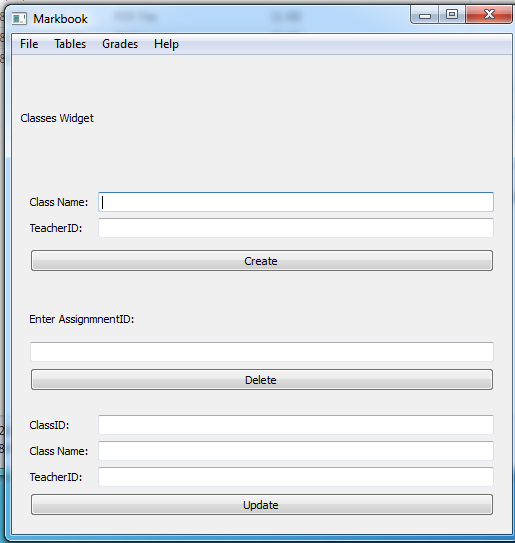
\includegraphics[width=\textwidth]{./Images/classes.png}
    \caption{The result of executing the print() function} \label{}
\end{figure}

\begin{figure}[H]
    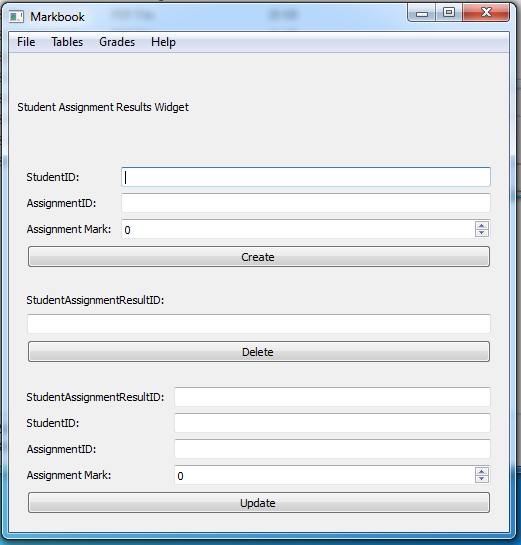
\includegraphics[width=\textwidth]{./Images/student assignments.png}
    \caption{Student Assignments Widget} \label{}
\end{figure}

\begin{figure}[H]
    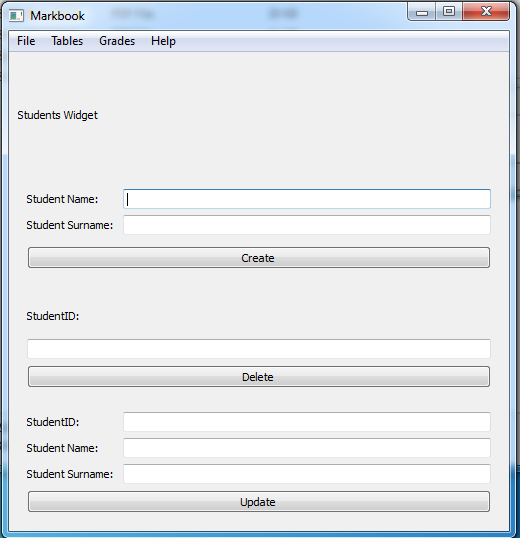
\includegraphics[width=\textwidth]{./Images/students.png}
    \caption{Students Widget} \label{}
\end{figure}

\begin{figure}[H]
    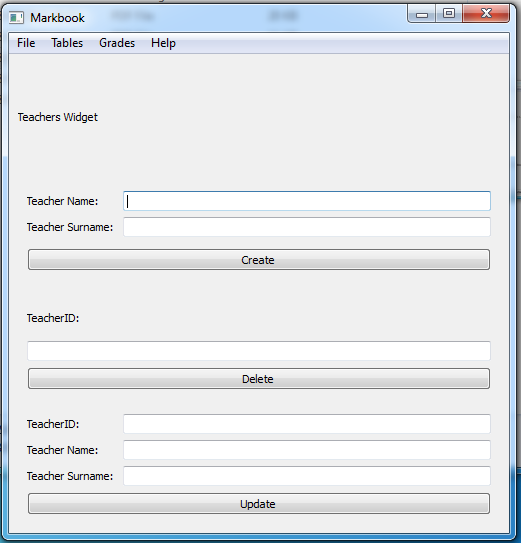
\includegraphics[width=\textwidth]{./Images/teachers.png}
    \caption{Teachers Widget} \label{}
\end{figure}

\begin{figure}[H]
    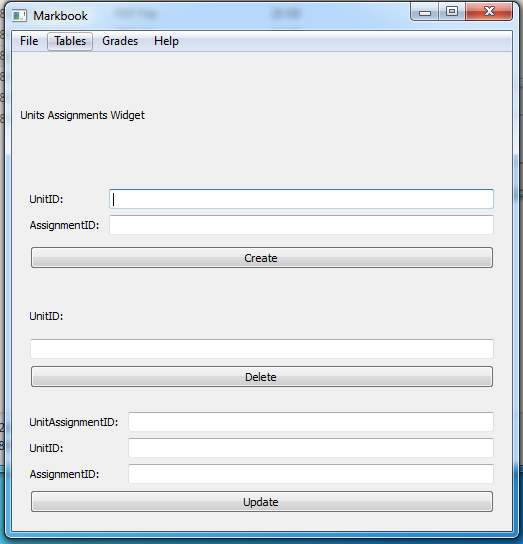
\includegraphics[width=\textwidth]{./Images/unit assignments.png}
    \caption{Unit Assignments Widget} \label{}
\end{figure}

\begin{figure}[H]
    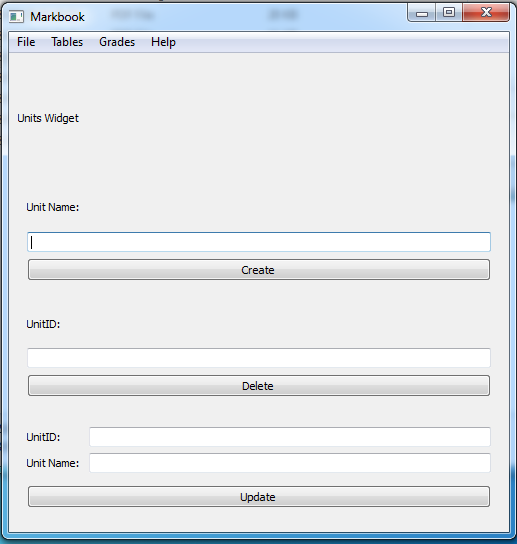
\includegraphics[width=\textwidth]{./Images/units.png}
    \caption{Units Widget} \label{}
\end{figure}
\subsection{ER Diagram}

\begin{figure}[H]
    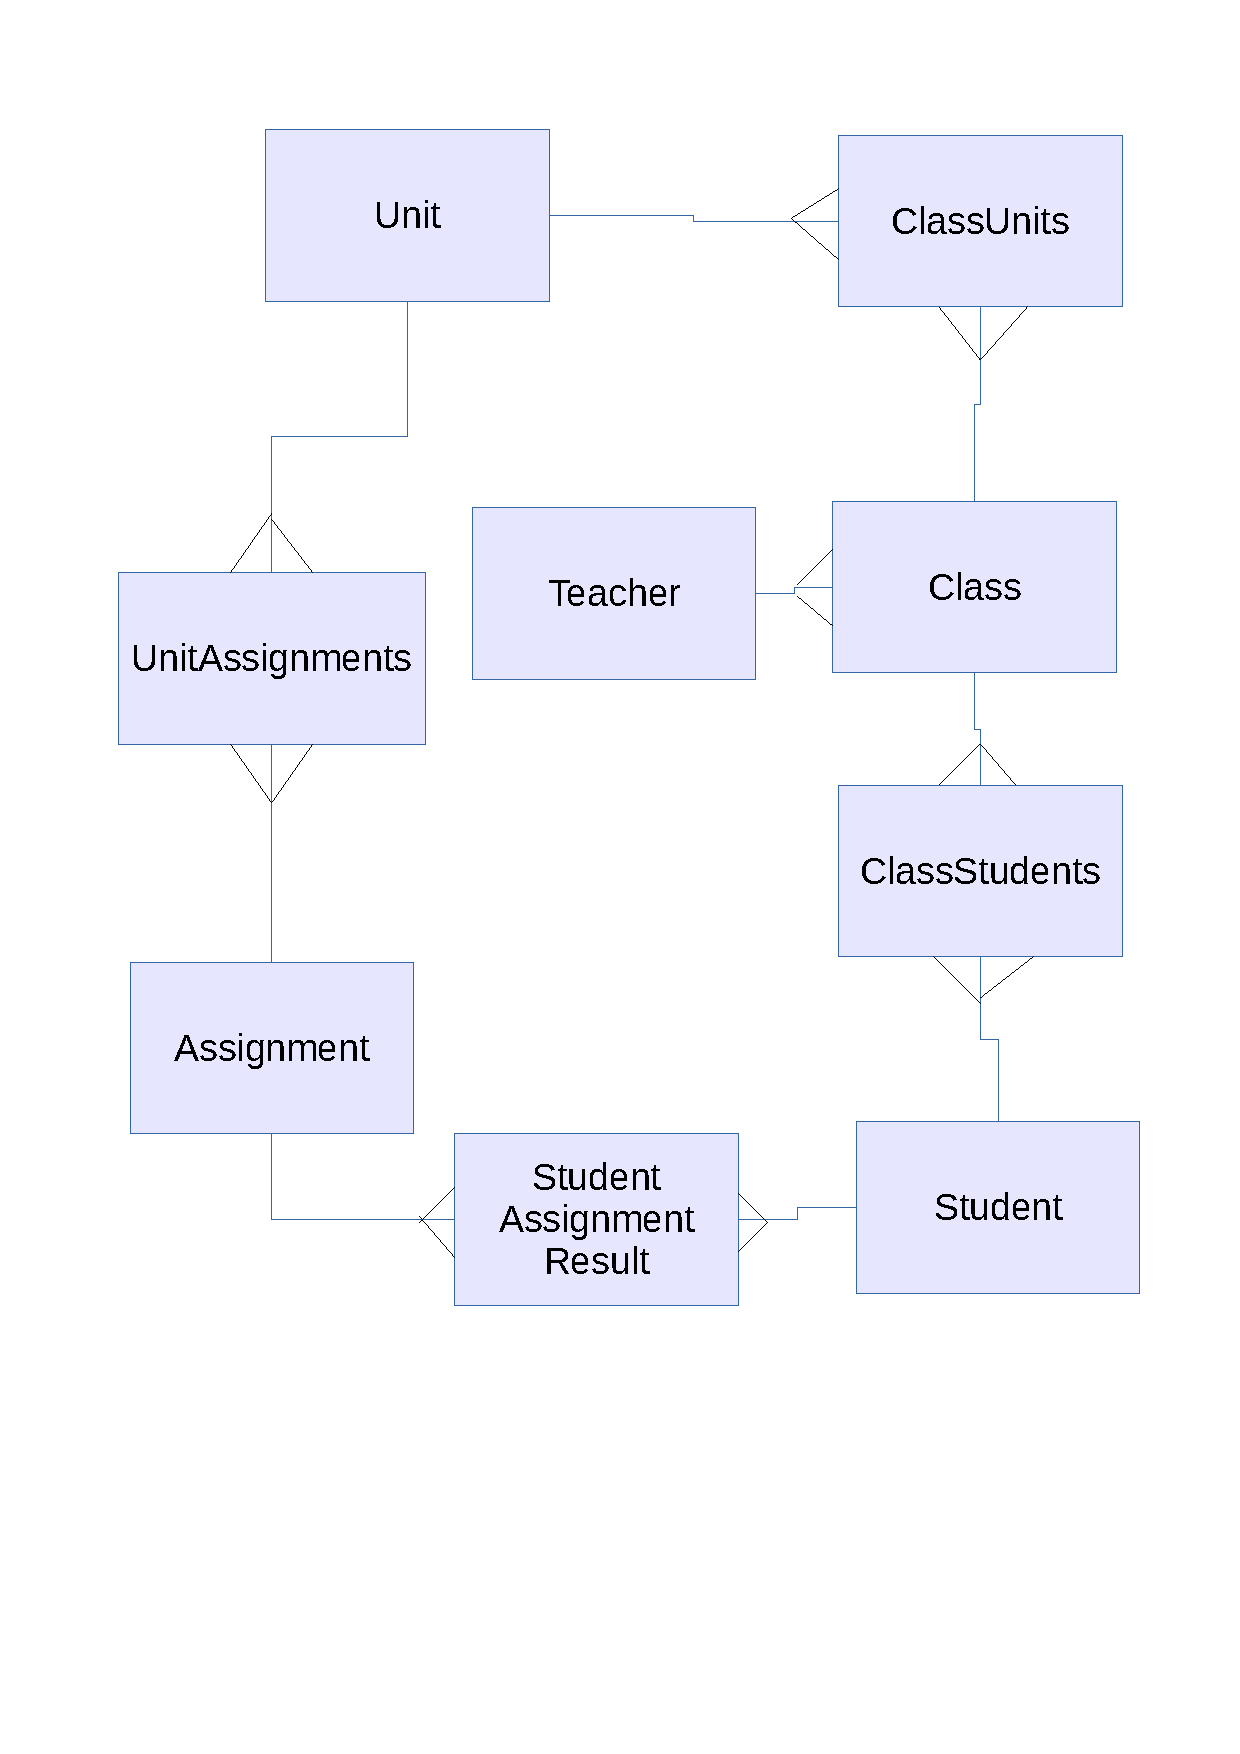
\includegraphics[width=\textwidth]{./Images/ER Diagram (Revised).pdf}
    \caption{} \label{}
\end{figure}

\subsection{Database Table Views}
Markbook fails to produce tables, although it is possible to view code which I implemented to produce tables in future Markbook versions. All of it is included under table_widget.py python file. 

\subsection{Database SQL}

\subsection{SQL Queries}
SQL Queries in Markbook are not complex and are very similar. Therefore, I will only explain one type of each query.

\subsubsection{find queries}
Those queries are used when PyQt tables are produced from the data in database. 
At this time, Markbook does not make a use of this query, but it will in future updates.
\begin{figure}[H]
    \pythonfile[firstline=55,lastline=59]{./Final/Markbook/SQLConnection.py}
    \caption{Select all data from ClassStudents table (query)} \label{}
\end{figure}

\subsubsection{insert queries}
Those queries are used when data is inserted into a database.
 
\begin{figure}[H]
    \pythonfile[firstline=86,lastline=91]{./Final/Markbook/SQLConnection.py}
    \caption{Insert AssignmentName and AssignmentMaxMark to Assignments (query)} \label{}
\end{figure}

\subsubsection{delete queries}
Those queries are used when a record is going to be deleted in a tabase.
\begin{figure}[H]
    \pythonfile[firstline=142,lastline=146]{./Final/Markbook/SQLConnection.py}
    \caption{Delete Assignment Query} \label{}
\end{figure}
This is an example of a delete query. All delete queries in Markbook are pretty much the same.
Record to be deleted is chosen by its ID. 

\section{Testing}
\subsection{Summary of Results}
I only managed to test navigation. Overall, navigation functions correctly I did not discover any issues when layouts were switched.

\subsection{Known Issues}
As I mentioned in analysis and design, Markbook should produce graphs and this section is missing. To my knowledge, FigureCanvas is a base class for graphs in python and is part of matplotlib module.

\section{Code Explanations}

\subsection{Difficult Sections}

\subsection{Self-created Algorithms}

\section{Settings}

\section{Acknowledgements}

\section{Code Listing}
\begin{landscape}
%include as many subsections as you have modules
%the code below can be uncommented and used to get a code section from a particular file
\begin{scriptsize}
\begin{landscape}
\subsection{CLI}
\begin{figure}[H]
    \pythonfile[firstline=1]{./Final/CLI/CLI.py}
    \caption{CLI.py)} \label{}
\end{figure}
\begin{figure}[H]
    \pythonfile[firstline=55,lastline=59]{./Final/CLI/start.py}
    \caption{start.py)} \label{}
\end{figure}
\subsection{Markbook with PyQt interface}

\begin{figure}[H]
    \pythonfile[firstline=1]{./Final/Markbook/main_window.py}
    \caption{main_window.py)} \label{}
\end{figure}

begin{figure}[H]
    \pythonfile[firstline=1]{./Final/Markbook/SQLConnection.py}
    \caption{SQLConnection.py} \label{}
\end{figure}

begin{figure}[H]
    \pythonfile[firstline=1]{./Final/Markbook/basic_widgets.py}
    \caption{basic_widgets.py} \label{}
\end{figure}

begin{figure}[H]
    \pythonfile[firstline=1]{./Final/Markbook/assignments_widget.py}
    \caption{assignments_widget.py} \label{}
\end{figure}

begin{figure}[H]
    \pythonfile[firstline=1]{./Final/Markbook/classes_widget.py}
    \caption{classes_widget.py} \label{}
\end{figure}

begin{figure}[H]
    \pythonfile[firstline=1]{./Final/Markbook/classStudents_widget.py}
    \caption{classStudents_widget.py} \label{}
\end{figure}

begin{figure}[H]
    \pythonfile[firstline=1]{./Final/Markbook/classUnits_widget.py}
    \caption{classUnits_widget.py} \label{}
\end{figure}

begin{figure}[H]
    \pythonfile[firstline=1]{./Final/Markbook/studentAssignmentResults_widget.py}
    \caption{studentAssignmentResults_widget.py} \label{}
\end{figure}

begin{figure}[H]
    \pythonfile[firstline=1]{./Final/Markbook/students_widget.py}
    \caption{students_widget.py} \label{}
\end{figure}

begin{figure}[H]
    \pythonfile[firstline=1]{./Final/Markbook/teachers_widget.py}
    \caption{teachers_widget.py} \label{}
\end{figure}

begin{figure}[H]
    \pythonfile[firstline=1]{./Final/Markbook/unitAssignments_widget.py}
    \caption{unitAssignments_widget.py} \label{}
\end{figure}

begin{figure}[H]
    \pythonfile[firstline=1]{./Final/Markbook/units_widget.py}
    \caption{units_widget.py} \label{}
\end{figure}

begin{figure}[H]
    \pythonfile[firstline=1]{./Final/Markbook/table_widget.py}
    \caption{table_widget.py} \label{}
\end{figure}


\end{landscape}
\end{scriptsize}
\end{comment}




